\documentclass[10pt]{article}
\usepackage[margin=0.72in]{geometry}
\usepackage{graphicx}
\usepackage{booktabs}
\setlength{\parindent}{0pt}
\setlength{\parskip}{5pt}
\begin{document}
\section*{n49 polynomial00: D5 checkpoint rank screen}
The local D5 attempt timed out after 21,621.6 recorded seconds without a degree-five certificate. The independent D4 checker accepted codimension at least 32,291; a fresh exact counter found two solutions. This retains last fall degree at least 5 for the named Boolean presentation.

Nine S3 checkpoint manifests were downloaded and hashed. Sequence 2 already recorded rank 59,351 in 59,353 working coordinates; sequences 3 through 9 retained the same rank. The worker only appends relation rows before echelonization, so rank cannot decrease. If this checkpointed worker later exports a candidate, its source computes codimension as $\mathrm{work}-\mathrm{rank}\leq 2$. The exact solution count is 2, so this instrument and checkpoint cannot satisfy the strict codimension-above-count degree-six test. It may kill the constant or fail instead. This screen is conditional on the recorded checkpoint state; it is not an upper bound on last fall degree.

\begin{center}
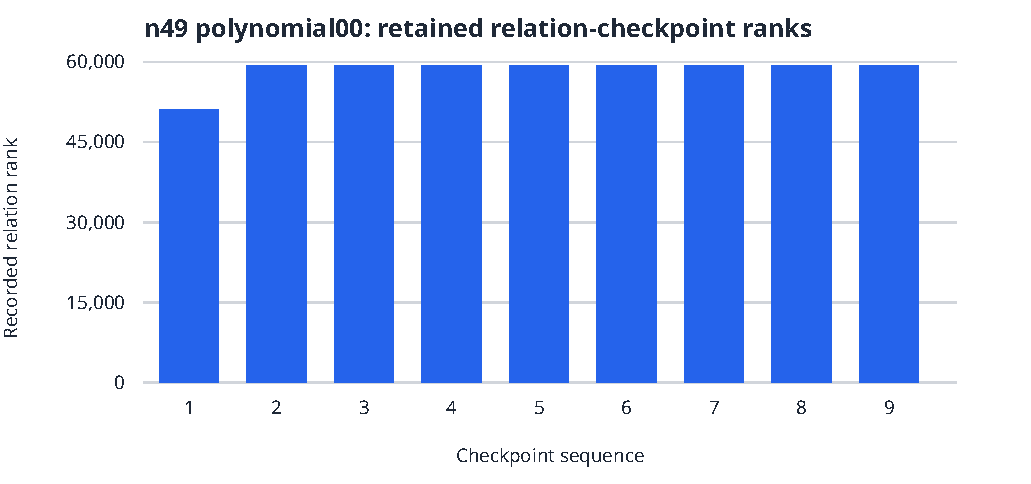
\includegraphics[width=0.96\linewidth]{checkpoint-rank.pdf}
\end{center}
\small{Recorded native ranks by immutable checkpoint sequence; no independent D5 certificate or timing comparison follows from this plot.}

\paragraph{Custody.} \texttt{readback.json} gives full SHA-256 reads for the retained local result and checker/count transcripts and for nine S3 manifests. It checks sequence, width, monotone rank, D4 acceptance, and exact count. The 440,622,032-byte sequence-9 snapshot object was not downloaded here; its manifest records its digest and publication readback.
\end{document}
